\documentclass[conference]{IEEEtran}
\IEEEoverridecommandlockouts
% The preceding line is only needed to identify funding in the first footnote. If that is unneeded, please comment it out.
\usepackage{cite}
\usepackage{amsmath,amssymb,amsfonts}
\usepackage{algorithmic}
\usepackage{graphicx}
\usepackage{textcomp}
\usepackage{xcolor}
\def\BibTeX{{\rm B\kern-.05em{\sc i\kern-.025em b}\kern-.08em
    T\kern-.1667em\lower.7ex\hbox{E}\kern-.125emX}}
\begin{document}

\title{Experimental investigation of forced convective heat transfer in cylindrical pipe flow\\
%{\footnotesize \textsuperscript{*}Note: Sub-titles are not captured in Xplore and should not be used}
%\thanks{Identify applicable funding agency here. If none, delete this.}
}

\author{\IEEEauthorblockN{Yoshinori Hattori}
\IEEEauthorblockA{\textit{Shibaura Institute of Technology, Mechanical Engineering}\\
Tokyo, Japan \\
md18060@shibaura-it.ac.jp}}

\maketitle

\section{Introduction}
Forced convective heat transfer in cylindrical pipe flow plays an important role in many technical cooling systems.
These coolant technology is used wide varaety of coolant applications such as electric devices, automotive, and plant factory.
Considering heat transfer issues, heat transfer coefficients are one of the most important numbers.

Much remains to be studied for providing experimental data for high Pramdlt number and laminar-to-turbulent transitional regime.
In this study, I focus on forced convective heat transfer in cylindrical pipe flow in particular high Pramdlt number and transitional regime.
Shell Heat Transfer Oil was used as a operating liquid.
%A 50/50vol\% mixture of water and glycole which is a typical liquid coolant in automotive applications were used as a operating fluid.


\section{state-of-art}
Figure. \ref{result} shows dimensionless heat transfer coeffcients from literature.
Gunielinski \cite{Gnienlinski2010} showed correlations for each flow regime, laminar and turbulent, respectively.
Morover, he presented transitional flow regime as a liner interpolation between laminar and turbulent flow.

\begin{figure}[htbp]
  \centering
  \vspace{4zh}
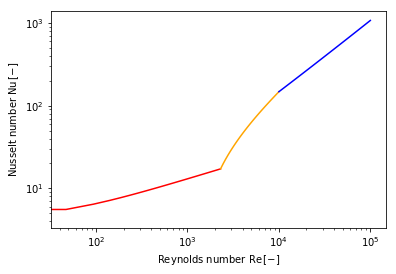
\includegraphics[width=0.47\textwidth,natwidth=400,natheight=200]{fig/result.png}
  \caption{Dimensionless heat transfer coefficients compared to literature data for Pr = 26. The red, yellow and blue lines are Gnielinski correlations for laminar, transitional and turbulent, respectively.}
  \label{result}
\end{figure}

Here, reliable prediction and experimental data are needed to predict heat transfer coefficients.
\textbf{Considering reliable prediction, uncertainty in Nusselt number is extremely important.}

\section{Uncertainty in Nusslet number}
It is nessesary to estimate the maximum possible error in the parameters evaluated from the measuring data.

Nusselt number is calcuretad from Equation \ref{Nu_calcuration}.
\begin{equation}
Nu=\frac{\dot{m} c_{p}(T_{1}-T_{0})}{\lambda (T_{w}-T_{1}) d\pi L}\label{Nu_calcuration}
\end{equation}

The uncertainty in Nusselt number is calcurated from Equation \ref{Nu_uncertainty1}.
\begin{equation}
Nu=\sqrt{\sum \left(\frac{\partial Nu}{\partial X_{i}} \Delta X_{i}\right)^{2}}\label{Nu_uncertainty1}
\end{equation}

Each parameter, X effects each parameters of Equation.\ref{Nu_calcuration}
Then, the mesurement uncertainty in Nusselt number leads to Equation \ref{Nu_uncertainty2}.

\begin{equation}
\begin{split}
&\frac{\Delta Nu}{Nu} =\frac{1}{Nu}\sqrt{\left(\frac{\Delta \dot{m}}{\dot{m}}\right)^{2}+\left(\frac{\Delta c_{p}}{c_{p}}\right)^{2}+\left(\frac{\Delta \lambda}{\lambda}\right)^{2}}\\
&\quad +\left(\frac{\Delta T}{T_{0}-T_{1}}\right)^{2}+\left(\frac{\Delta T(T_{0}-T_{w})}{(T_{0}-T_{1})(T_{1}-T_{w})}\right)^{2}+\left(\frac{\Delta T}{T_{1}-T_{w}}\right)^{2}\\\label{Nu_uncertainty2}
\end{split}
\end{equation}

I estimated mesurement error of mass flow and temperature sensors are 0.20E-3$\dot{m}$, 0.2K.
Specific heat capacity and heat conductivity are calcurated from fluid properties, temperature dependance.
Specific heat capacity and heat conductivity are function of temperature as shown in Equation \ref{specific_heat_capacity} and \ref{heat_conductivity}.
\begin{equation}
C_{p} = 818 + 3664T \times 10^{-3} \label{specific_heat_capacity}
\end{equation}
\begin{equation}
\lambda = 0.157 - 7.328T \times 10^{-5} \label{heat_conductivity}
\end{equation}
Therefore, mesurement error of specific heat capacity Cp and heat conductivity $\lambda$ are 0.73 and 1.56E-5, respectively.

Here, I picked up two experimental data.
Shell Heat Transfer Oil was used as a operating liquid.
Table\ref{experimental_result} shows experimental results for Re=4275, Pr=26 and Re=6172, Pr=27, respectively.

\begin{table}[h]
 \caption{Esperimental results for Re=4275, Pr=26 and Re=6172, Pr=27.}
 \label{experimental_result}
 \centering
\begin{tabular}{llllllll}
\hline
       & Re   & Pr & T0    & T1    & Tw     & Massflow & Nu   \\ \hline
CASE A & 4275 & 26 & 438.25 & 446.85 & 472.45 & 0.054    & 56.0 \\
CASE B & 6172 & 25 & 452.87 & 452.87 & 478.97 & 0.073    & 81.6
\end{tabular}
\end{table}

The resulting uncertainty in nusselt numbers were analyzed for each of 2 data points.
Table\ref{uncertainty_in_Nusselt_number} summrizes uncertainty in Nusselt number of each data points.

\begin{table}[h]
 \caption{Uncertainty in Nusselt number.}
 \label{uncertainty_in_Nusselt_number}
 \centering
\begin{tabular}{clc}
\hline
\multicolumn{3}{l}{Uncertainty in Nusselt number}         \\ \hline
CASE   & \multicolumn{1}{c}{Flow regime, Pr} & Nusselt number \\ \hline
CASE A & Re = 4275, Pr = 26              & 4\%            \\
CASE B & Re = 6172, Pr = 25              & 3\%           
\end{tabular}
\end{table}

Figure. \ref{uncertainty} shows heat transfer coefficients compared to literature data for transitional regime, Pr = 26.
Two data shows good agreement with calcuration method for transitional regime proposed by Gunielinski \cite{Gnienlinski2010}.

\begin{figure}[htbp]
  \centering
  \vspace{5zh}
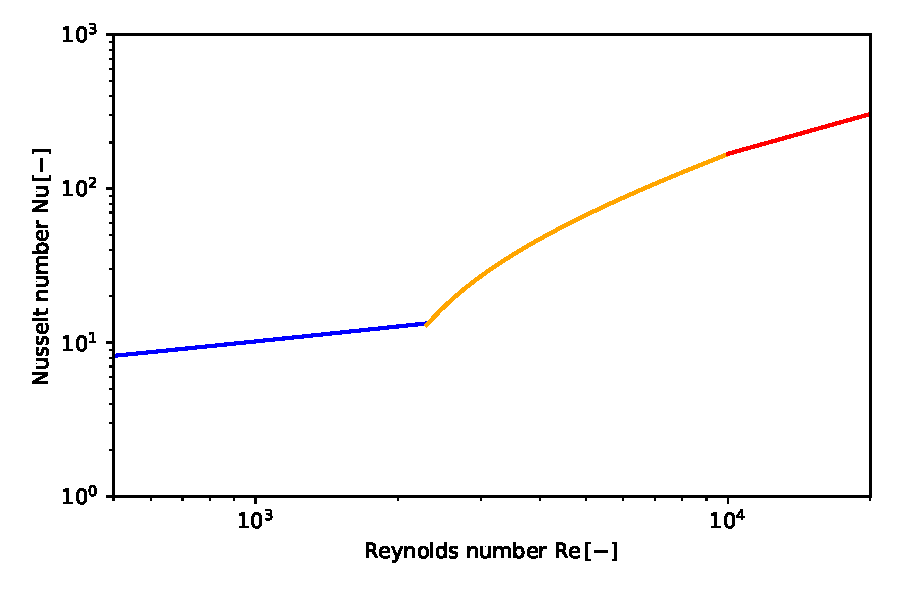
\includegraphics[width=0.47\textwidth,natwidth=400,natheight=200]{fig/uncertainty.pdf}
  \caption{Dimensionless heat transfer coefficients compared to literature data for Pr = 26.}
  \label{uncertainty}
\end{figure}


\section{Purpose of the solution}

Table \ref{order} shows the orders of each terms in Equation \ref{Nu_uncertainty2}.
From this comprehensive result, temperature term is several orders of magnitude larger than others.
Therefore, temperature mesurement is strongly inflected to mesurement uncertainty.
According to this analisis, careful selections of temperature sensors are needed.

\begin{table}[h]
 \caption{Oders of each terms in Equation \ref{Nu_uncertainty2}.}
 \label{order}
 \centering
 \begin{tabular}{ccccc}
\hline
      & Mass flow & Specific heat capacity & Lambda & Temperature \\ \hline
Order & O (-8)    & O (-8)                 & O(-8)  & O(-4)      
 \end{tabular}
\end{table}


%\section{Measurement uncertainty}
%The uncertainty of measurement was analyzed by using ``Guide to the Expression of Uncertainty in Measurement``(GUM).
%\\

\begin{thebibliography}{00}
%\bibitem{Frank} Frank P. Incropera, David P. DeWitt, ``Fundamentals of Heat and Mass Transfer,'' 4th edition., WILEY, 1996.
\bibitem{Gnienlinski2010} V. Gnienlinski, ``Heat Transfer in Laminar Flow,'' VDI Heat Atlas, second ed., Springer Verlag, 2010 (Chapter Ga 1-7), Section 3.
%\bibitem{Petukhov1958} B.S. Petukhov, V.V. kirillov, Teploenergetika 4 (1958) 91-98.
\bibitem{Bertsche2016} Dirk Bertsche, Paul Knipper, Thomas Wetzel, ``Experimental investigation on heat transfer in laminar, transitional and turbulent circular pipe flow,'' International Journal of Heat Transfer, 95 (2016) 1008-1018.
\bibitem{Christphan2018} Christphan, ``Title of paper if known,'' unpublished, 2018.
%\bibitem{Konakov1954} Konakov, ``Eine neue Formel fr den Reibungskoezienten glatter Rohre,'' Bericht der Akademie der Wissenschaften der UDSSR 51.7, 503-506.

% \bibitem{b5} R. Nicole, ``Title of paper with only first word capitalized,'' J. Name Stand. Abbrev., in press.
% \bibitem{b6} Y. Yorozu, M. Hirano, K. Oka, and Y. Tagawa, ``Electron spectroscopy studies on magneto-optical media and plastic substrate interface,'' IEEE Transl. J. Magn. Japan, vol. 2, pp. 740--741, August 1987 [Digests 9th Annual Conf. Magnetics Japan, p. 301, 1982].
% \bibitem{b7} M. Young, The Technical Writer's Handbook. Mill Valley, CA: University Science, 1989.

%\bibliography{junsrt}
%\bibliography{project_forced_convective@Graz.bib}

\end{thebibliography}
%\vspace{12pt}
%\color{red}
%IEEE conference templates contain guidance text for composing and formatting conference papers. Please ensure that all template text is removed from your conference paper prior to submission to the conference. Failure to remove the template text from your paper may result in your paper not being published.

\end{document}
